\documentclass[border=10pt]{standalone}
\usepackage{graphicx} % Required for inserting images
\usepackage{tikz}
\usetikzlibrary{automata, positioning, arrows}

\begin{document}

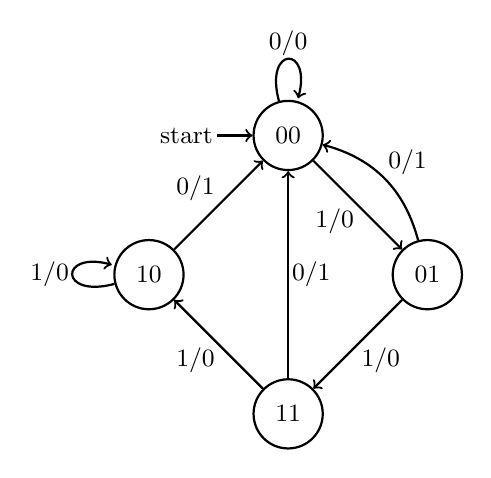
\begin{tikzpicture}[
    node distance=2.5cm,
    thick,auto,
    every node/.style={font=\small, inner sep=1pt} % Make labels smaller and closer to edges
]
% draw the states
\node[state,initial] (s_0) {$00$}; % note the semicolon
\node[state] (s_1) [below right of=s_0] {$01$};
\node[state] (s_2) [below left of=s_1] {$11$};
\node[state] (s_3) [above left of=s_2] {$10$};
% draw the edges
\path[->] 
(s_0) edge node [swap] {1/0} (s_1)
edge [loop above] node [swap] {0/0} (s_0)
(s_1) edge [bend right] node [swap] {0/1} (s_0)
edge node {1/0} (s_2)
(s_2) edge node [swap] {0/1} (s_0)
edge node {1/0} (s_3)
(s_3)
edge [loop left] node {1/0} ()
edge node {0/1} (s_0)

; % note the semicolon
\end{tikzpicture}

\end{document}